
\documentclass[border=3pt,tikz]{standalone}
\usepackage[utf8]{vietnam}
\usetikzlibrary{calc,angles,intersections,shapes.geometric,arrows,decorations.markings,arrows.meta,patterns.meta,patterns}
\usepackage{tikz-3dplot,pgfplots}
\pgfplotsset{compat=1.15}
\usepgfplotslibrary{polar}
\usepackage{amsmath}
\begin{document}
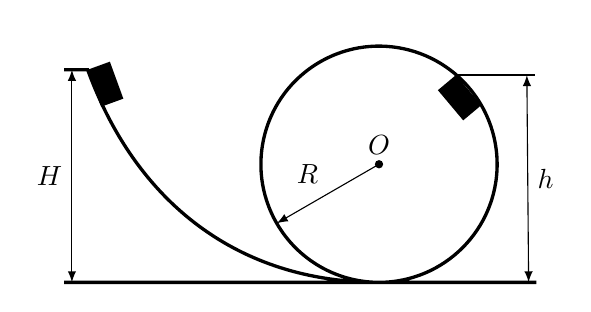
\begin{tikzpicture}[>=latex]
	\coordinate (A) at (0,2.7);
	\coordinate (B) at (0,0);
	\coordinate (C) at (6,0);
	\coordinate (O) at (4,1.5);
	\draw[very thick] (A)--++(0:.3)coordinate(X)to[out=-70,in=180] (4,0)arc(-90:30:1.5)coordinate(M)arc(30:210:1.5)coordinate(N)arc(210:270:1.5) (B)--(C);
	\fill (M)--++(220:.3)--++(130:.5)--++(40:.3)coordinate(P)--cycle (X)--++(20:.3)--++(-70:.5)--++(-160:.3)--cycle (O)node[above]{$O$}circle(1.5pt);
	\draw (P)--++(0:1)coordinate(D);
	\draw[<->] ([xshift=.1cm]A)--([xshift=.1cm]B)node[left,pos=.5]{$H$};
	\draw[<->] ([xshift=-.1cm]C)--([xshift=-.1cm]D)node[right,pos=.5]{$h$};
	\draw[->] (O)--(N)node[above left,pos=.5]{$R$};
\end{tikzpicture}
\end{document}